%%%%%%%%%%%%%%%%%%%%%%%%%%%%%%%%%%%%%%%%%%%%%%%%%%%%%%%%%%%%%%%%%%%%%%%%%%%%%%%%%
%
% Purpose:  Verification part of V&V for the SolarBeta model
%
% 
%
%%%%%%%%%%%%%%%%%%%%%%%%%%%%%%%%%%%%%%%%%%%%%%%%%%%%%%%%%%%%%%%%%%%%%%%%%%%%%%%%

% \section{Verification}

%%% code imported from old template structure
%\inspection{<Name of Inspection>}\label{inspect:<label>}
% <description> to satisfy  
% requirement \ref{reqt:<label>}.

Given the simplicity of the model, a single simulation can be used for all of the verification and validation tests.  The initialization of some aspects, such as solar and lunary gravity, is redundant for some tests, but having one simulation simplifies that validation greatly.  The simulation uses the DE405 ephemeris model to compute planetary ephemeris and simulates an orbital body as a ``falling rock'' orbiting the Earth for up to a year.

\test{Long-Term Behavior}
\label{test:solarbetalongterm}
\begin{description}
\item{Purpose:} \\
The purpose of this test is to verify the solar beta angle characteristics
and accuracy over a period of time. 

\item{Requirements} \\
The succesful outcome of this test, together with the validation Test~\ref{test:solarbetacompare} satisfy requirement~\ref{reqt:SolarBeta}.
\item{Procedure:} \\
The simulation is run for one
year with different orbital inclinations and gravity modeled as
spherical or 8x8, with solar and lunar gravitational perturbations on and off.

\item{Predictions:}
\begin{enumerate}
 \item {Equatorial orbit, spherical gravity} \ \newline
The Solar Beta will show a single cycle of variation associated with the orbit (which has a fixed-orientation in an inertial frame) passing once around the sun.  The magnitude of that oscillation should be equal to the tilt of Earth's axis with respect to the ecliptic, $23.44^\circ$
\item{Inclined orbit, $23.4^\circ$, non-spherical gravity} \ \newline
The Solar Beta will oscillate more rapidly as the orbital plane precesses in the non-spherical gravitational field.  This should cause an additional oscillation of $23.4^\circ$ due to the orbital inclination \textit{on top of} the annual variation due to the orientation of the equator as expected from the previous case.  
\item{Inclined orbit, $51.6^\circ$, non-spherical gravity} \ \newline
This case should be comparable to the previous case, with a longer-term precession, and larger oscillation about the equatorial oscillation seen in the first case. 
\item{Inclined orbit, $23.4^\circ$, spherical gravity, lunar and solar gravitational perturbation on} \ \newline
Several cases were run for comparison
\begin{enumerate}
 \item Inclined orbit, $23.4^\circ$,  with spherical gravity.
 \item Inclined orbit, $23.4^\circ$,  with spherical gravity, and the addition of lunar gravitational perturbations.
 \item Inclined orbit, $23.4^\circ$,  with spherical gravity, and the addition of lunar and solar gravitational perturbations.
\end{enumerate}
All of these should show an annual variation, with small oscillations induced by the gravitational perturbations to the orbit. 

\end{enumerate}

\item{Results:}
\begin{enumerate}
 \item {Equatorial orbit, spherical gravity} \ \newline
Data is as expected, see Figure~\ref{fig:solbeta123} for comparison of cases 1, 2, and 3.
\item {Inclined orbit, $23.4^\circ$, non-spherical gravity} \ \newline
Data is as expected, see Figure~\ref{fig:solbeta123} for comparison of cases 1, 2, and 3.  The figure shows an appropriately scaled short-period oscillation superposed on the long-period (annual) oscillation.
\item {Inclined orbit, $51.6^\circ$, non-spherical gravity} \ \newline
Data is as expected, see Figure~\ref{fig:solbeta123} for comparison of cases 1, 2, and 3.  The figure shows an appropriately scaled short-period oscillation superposed on the long-period (annual) oscillation.  The short-period oscillation has larger period than for the less inclined orbit.  Similar runs for orbits inclined at 70, 85, and 90 degrees continued the trend, with more pronounced variation in the Solar beta angle, and longer duration precession, gradually slowing until no orbital precession was evident at 90 degrees.
\item{Gravitational Perturbations} \ \newline
The effect of graviational perturbations on the orientation of the orbit are small; the addition of lunar perturbations has more effect than the addition of solar perturbations.
\end{enumerate}
\end{description}

\begin{figure}[!ht]
  \begin{center}
        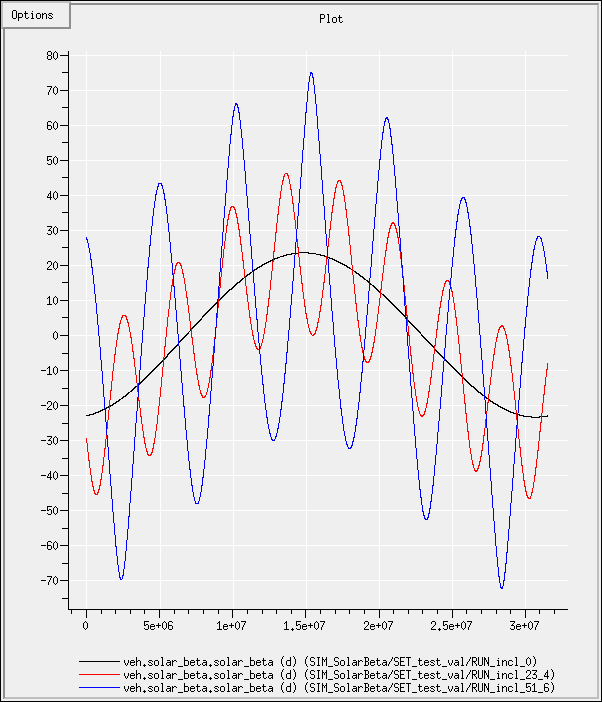
\includegraphics[width=80mm]{figures/solbeta123.jpg}
        \caption{The variation of Solar Beta with time for the first three test cases.  These are all circular orbits with orbital inclinations of 0, 23.4, and 51.6 degrees respectively} 
        \label{fig:solbeta123}
  \end{center}
\end{figure}
